\chapter{Carrier Recovery}

Carrier recovery is a processes used in coherent demodulation where the phase
and the frequency of the transmitter carrier wave are recovered by the receiver
and thus after having such information it is possible to extract the information
in the transmitted signal.\\
Considering that the phase and frequency of the transmitted wave probably will 
be affected by noise, it is not a straight-forward method, it includes filtering
and usually feedback systems to correct the erros in phase or frequency caused
by the noise.\\
This chapter aims in the brief exploration of some techniques used for carrier
recovering, such as Phase locked loops, costas loop and others.\\

\section{Phase-Locked Loop (PLL)}
\label{sec:pll}

Phase-locked Lopp is a kind of feedback system, which has been extensively used
in communications sytems and other applications which require frequency
synthesis.\\
The Phase-Locked Loop is composed by three basic components \ref{fig:pll}:

\begin{enumerate}
    \item A phase detector (PD).
    \item A loop filter.
    \item A voltage-controlled oscillator (VCO).
\end{enumerate}

As it can seen in the figure \ref{fig:pll} the phase-locked loop is a feedback
system whose main goal is to make the output signal the same as the input
signal. Basically the phase detector compares the phase of the input signal
against the pahse of the VCO output, then the PD output is inputed in the loop
filter whose output is the voltage that controls the VCO. The output of the
phase detector is the phase error between the input signal and the VCO and the
output of the loop filter outputs the control voltage to the VCO.\\

When the loop is locked, teoretically, the output frequency is the same as the
input frequency, but to maintain the control voltage necessary to lock it is
needed a nonzero output to the phase detector, thus the pll operates with some
phase error, but this tends to be small.\\

Pll makes simple to syntethize frequencies with a pll and do operations 
of analog modulation and demodulation, these applications willbe briefly 
discussed later.


\begin{figure}[htbp]
    \centering
    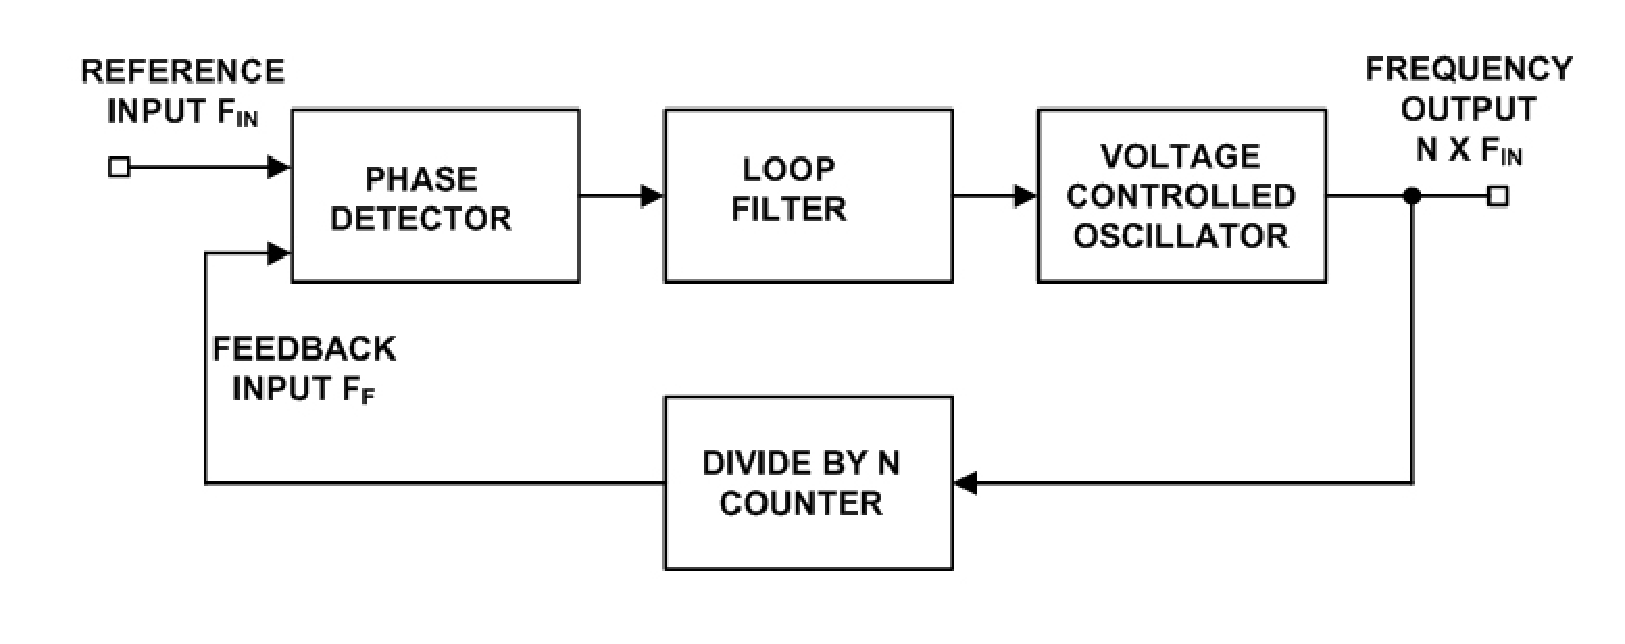
\includegraphics[width=0.65\textwidth]{./figures/pll.eps}
    \caption{ Basic PLL scheme
    \label{fig:pll}}
\end{figure}

\subsection{PLL Fundamentals}
Considering a basic pll scheme as shown in figure \ref{fig:pll2} we can see that
the input signal has a pahse of $\theta_i(t)$ and the VCO output has a phase of
$\theta_o(t)$. Assuming that the loop is locked and the phase detector is
linear, the ouput of the PD is proportional to the phase difference between its
inputs, thus,

\begin{equation}
    v_d = K_d(\theta_i - theta_o)
    \label{eq:pdout}
\end{equation}

where $k_d$ is the PD gain factor and its unity is volt/radian.\\

The $v_d$ is filtered by the loop filter, supressing noise and high frequency
signal components, the filter also contributes for the determination of the
dynamic performance of the loop. The filter transfer function is given by
$F(s)$.

Frequency output of the VCO is determined by the input $v_c$ and since frequency
is the derivative of the phase, the operation in the VCO can be described by,

\begin{equation}
    L[\frac{d\theta_o(t)}{dt}] = s\theta_o(s)=K_oV_c(s)
    \label{eq:vco}
\end{equation}

\begin{figure}[htbp]
    \centering
    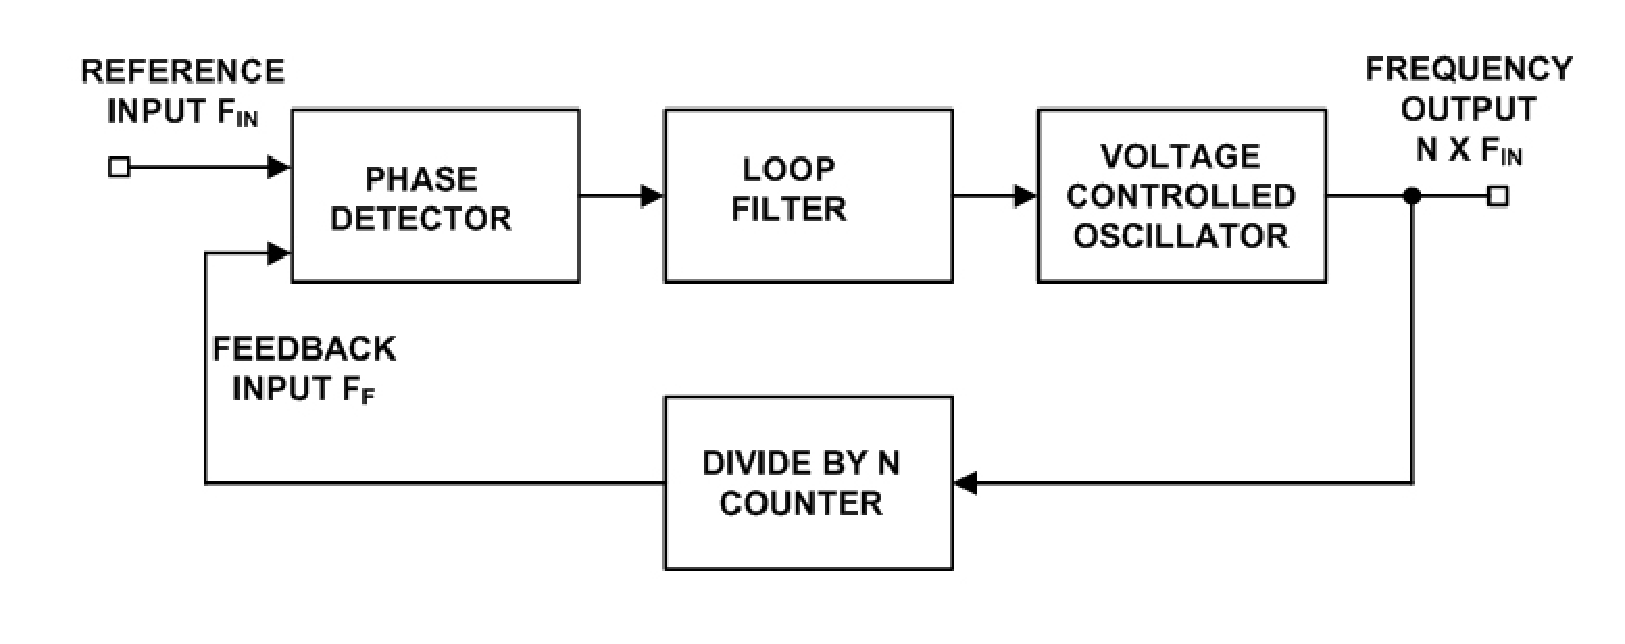
\includegraphics[width=0.65\textwidth]{./figures/pll.eps}
    \caption{ PLL
    \label{fig:pll2}}
\end{figure}

we can see that the output of the VCO is linearly related to the integral of the
control voltage.\\

Using laplace notation it is possible to stablish some basic equations to
describe the loop components behavior,

\begin{equation}
    V_d(s)=K_d[\theta_i(s) - \theta_o(s)]
    \label{eq:vd}
\end{equation}

\begin{equation}
    V_c(s)=F(s)V_d(s)
    \label{eq:vc}
\end{equation}

\begin{equation}
    \theta_o(s)=\frac{k_oV_c(s)}{s}
    \label{eq:thetao}
\end{equation}

The combination of these equations \ref{eq:vd} \ref{eq:vc} \ref{eq:thetao}
results in the basic loop equations:


\begin{equation}
    H(s)= \frac{\theta_o(s)}{\theta_i(s)}=
    \frac{K_oK_dF(s)}{s + K_oK_dF(s)}
    \label{eq:gentf}
\end{equation}

\begin{equation}
    \frac{\theta_i(s)-\theta_o(s)}{\theta_i(s)}=
    \frac{\theta_e(s)}{\theta_i(s)}=
    \frac{s}{s+K_oK_dF(s)}=1-H(s)
    \label{eq:pherr}
\end{equation}

\begin{equation}
    V_c(s)=\frac{sK_dF(s)\theta_i(s)}{s+K_oK_dF(s)}=
    \frac{s\theta_i(s)}{K_o}H(s) 
    \label{eq:vchs}
\end{equation}

Where:

\begin{itemize}
    \item $H(s)$ is the closed-loop transfer function
    \item $\theta_e$ is the phase error 
\end{itemize}

Based on the equantions which describe the behavior of the components in the 
phase-locked loop we can classify the pll based on the order of the transfer 
function associated with the loop. This classification is based upon the nunmber 
of perfect integrators ($\frac{1}{s}$) present in the transfer function.

\begin{itemize}
    \item First order loop.
    \item Second order loop.
    \item Third and higher order loop.
\end{itemize}

\subsubsection{First Order Loop}

The first order loop is the simplest implementation of a phase-locked loop,
where the loop filter is ommited, thus $F(s)=1$

\begin{equation}
    H(s)= \frac{K_oK_d}{s + K_oK_d}=
    \frac{K}{s + K}
    \label{eq:tf1st}
\end{equation}

Where:
\begin{itemize}
    \item $K = K_oK_d =K_v$;
\end{itemize}

\subsubsection{Second Order Loop}

The second order loop

\subsubsection{Third an Higher Order Loops }

\subsection{PLL Components}

\subsection{tracking}




